\chapter{Literature Review}
Queues with scheduled arrivals are widely studied. There is a large body of literature studying the potential of appointment systems to reduce customer waiting times and waiting room congestion. This research is essential as health care providers in particular are under a great deal of pressure to improve service quality and efficiency \citep{Goldsmith}.  Before we explore the detail of this thesis, it is important to review some of the papers that study this problem.

\citet{Fomundam}, and \citet{Cayirli} provide comprehensive surveys of research on appointment scheduling. Most of the papers on scheduled arrivals can be classed into two categories. Those that design algorithms to determine schedules, and those that evaluate schedules using simulation. While simulation studies can easily model complicated customer flows, queuing models often provide more generic results than simulation \citep{Green}.

The foundation paper on modeling queues with scheduled arrivals is \citet{Bailey}. Bailey proposes that customers' waiting times can be reduced without a significant increase in the server's idle time. The Bailey rule, which is commonly referenced in literature, is that customers should be scheduled to arrive at fixed intervals with two customers scheduled to arrive at the start of service. Bailey randomly generates a series of independent service times and finds that a great deal of time wasted by customers can be reduced without a significant increase in the server's idle time. Under the Bailey rule, customers with late appointments will wait longer than those with early appointments. This lack of uniformity might be perceived as unfair and thus an undesirable property of a schedule. 

\citet{Pegden} extend Bailey's paper. They present an algorithm to iteratively determine the optimal arrival times of $n$ customers that need to be scheduled. The optimal arrival times are those that minimise a linear combination of the expected customers' waiting time and the expected server's total availability time.

Pegden and Rosenshine prove that their objective function is convex for $n \leq 4$, thus their algorithm finds the optimal schedule. While they conjecture that the objective function is convex for all $n$, it has not been proven. Nevertheless, we refer to the times returned by their algorithm as `optimal times' throughout this thesis. This is both for simplicity and because we believe that they are in fact optimal.

\citet{Stein} apply Pegden and Roshenshine's model to obtain numerical results for situations with more than three customers. The optimal times between successive customers become near constant as $n$ grows. This is the often observed dome-shape. Figure~\ref{fig:Lit_Dome_Shape} plots several examples of this dome shape. Optimal interarrival times exhibit a common pattern where they initially increase towards the middle of a session, and then decrease. This figure will be explained more clearly in Chapter~\ref{chap:Static}.
\begin{figure}[htb]
	\centering
	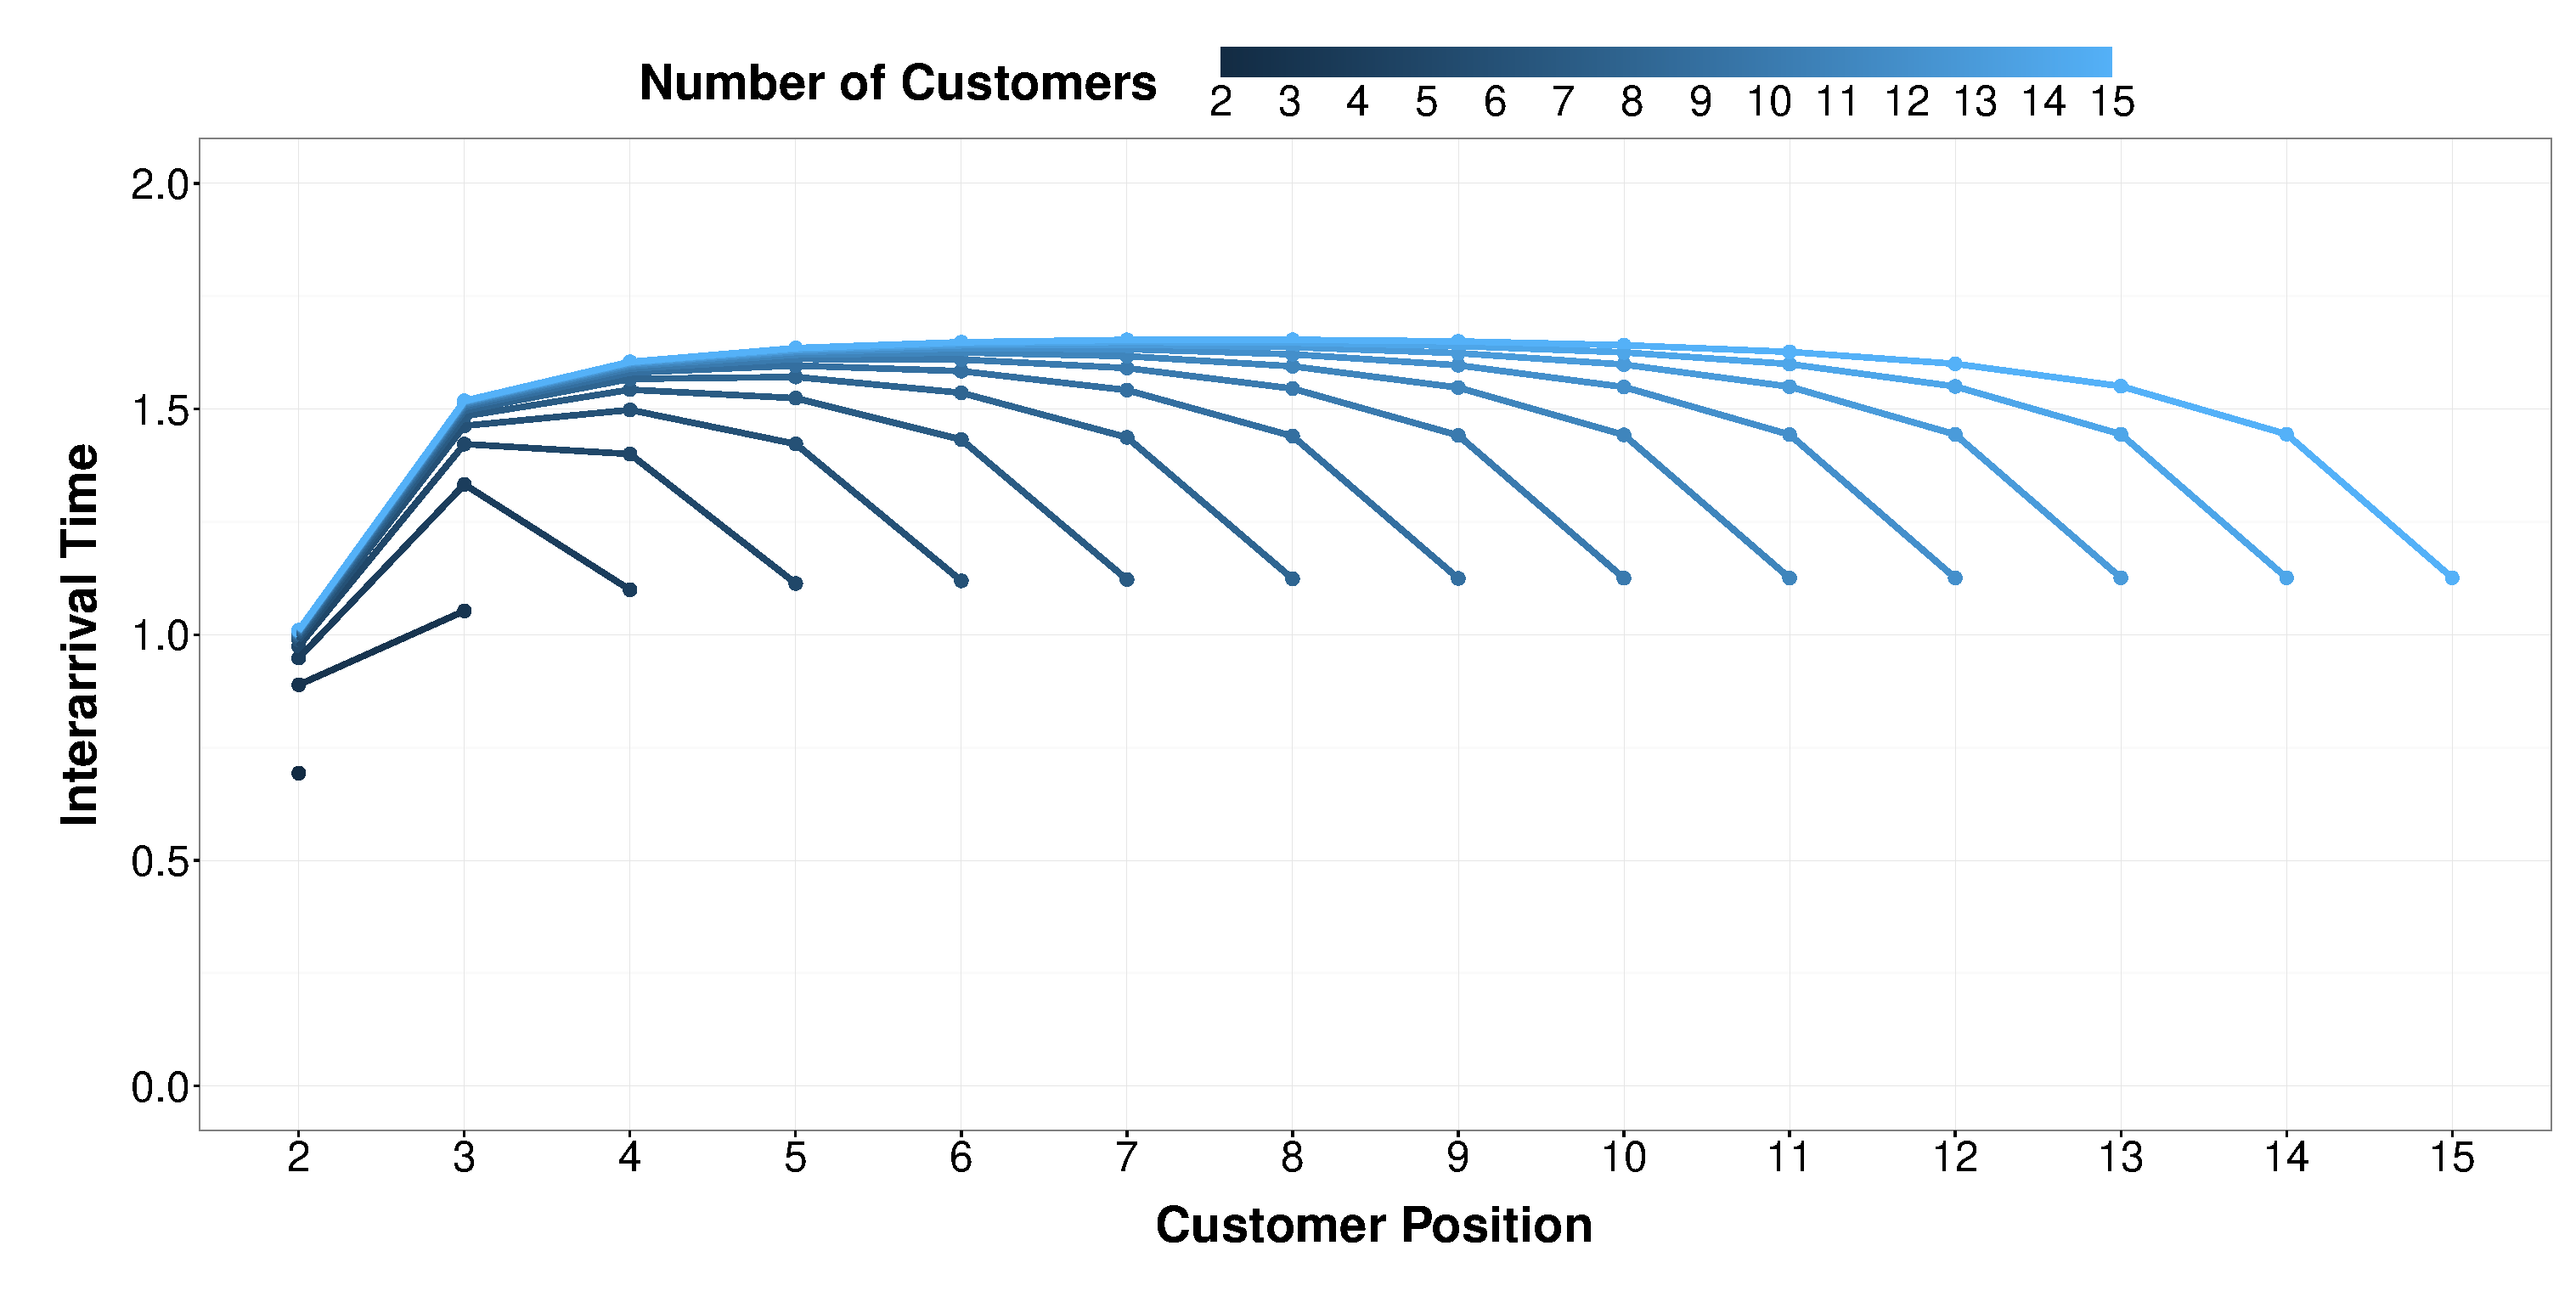
\includegraphics[width = 0.85\textwidth]{Static_Line_Interarrival_Num.eps}
	\caption{Optimal interarrival time for each customer after the first customer showing the dome-shapes as found by \citet{Stein}. Figure is explained more clearly in Chapter~\ref{chap:Static}. Figure generated assuming $\mu = 1$ and $\gamma = 0.5$. Each line is plotted for a given number of customers ($n$). The lightest line is the optimal schedule for $15$ customers. As $n$ decreases, the lines become darker.}
	\label{fig:Lit_Dome_Shape}
\end{figure}

Stein and C\^{o}t\'{e} simplify their model by requiring the intervals between arriving customers to be constant. This commonly studied restriction makes the model more easily applicable in practice, and more computationally efficient to solve for a large number of customers.

Stein and C\^{o}t\'{e} apply queuing theory results to solve the model for the optimal arrival interval assuming the queue reaches its steady state distribution. This assumption greatly reduces the computation required. However, in practice it is common to find services that never reach steady state. \citet{Babes} attempt to apply steady state queuing theory, but find their results tend to be very different from those observed in real operation. Many real-world services involve scheduling a relatively small number of customers (e.g., less than 30 customers). Thus, steady state behaviour is not explored in this thesis.

These key papers by Bailey, Pegden and Rosenshine, and Stein and C\^{o}te provide the basis for a more realistic exploration of health care systems. \citet{Delaurentis} highlight that customer no-shows can lead to a waste of resources. \citet{Mendel} incorporates the probability of a customer not showing up into the model presented by Pegden and Rosenshine. Unsurprisingly, no-shows lead to lower expected waiting times for customers who do show up.

The presence of walk-ins (regular and emergency) can disrupt a schedule. \citet{Gupta} propose a system where non-routine requests are superimposed on top of routine scheduled requests. \citet{Fiems} investigate the effect of emergency requests on the waiting times of scheduled customers. Fiems et al. model a system with deterministic service times and discrete time. Despite this research, Cayirli and Veral suggest that walk-ins are neglected in most studies. Further research could investigate their effect on optimal arrival times.

\citet{Mondschein} observe that the majority of the literature assumes that demand is exogenous and independent of customers' waiting times. These papers assume the total number of customers is fixed and independent of waiting times. The vast majority of servers are now private (including medical servers), so face competitive environments. Mondschein and Weintraub thus present a model where demand depends on the customers' expected waiting time.

Few authors attempt to model a dynamic schedule. \citet{Wang} considers the problem of scheduling a new customer when there are already a number of customers with fixed scheduled arrival times. The aim is to determine the optimal arrival time for the new customer such that the objective function remains optimal. However, Wang is criticised for not having a truly dynamic model \citep{Erdogan}. The initial scheduling of the customers ignores the possibility of an additional customer needing to be scheduled.

Simulation is a useful tool to analyse the effectiveness of appointment policies. \citet{Kao} use simulation to compliment their results obtained from queuing theory. \citet{Ho} study the performance of eight different appointment rules under different scenarios. They find that no rule will perform well under all circumstances.

Case studies can test the real world applications of an appointment system. While they lack generalisation, they are necessary to compliment the theoretical research. \citet{Rockart} show that individual block systems lead to more punctual doctors and patients, and less no-shows. \citet{Walter} indicates that the grouping of inpatients and outpatients results in a substantial reduction in the doctor's idle time.

Unfortunately, \citet{Cayirli} lament that despite much published work, the impact of appointment systems on outpatient clinics has been limited. Doctors are often unwilling to change their old habits. \citet{O'Keefe} have their proposed appointment system of classifying patients rejected by staff. \citet{Huarng} are unable to implement their system due to staff resistance. \citet{Bennett} find their recommendations are not implemented successfully. Future research should attempt to develop models that will be accepted and implemented in real health care services.
